% Printed 92--101. Continuation from printed 91.
\clearpage
\noindent 92\hfill POSTHUMOUS PAPERS.\hfill\mbox{}\par
\[
\begin{aligned}
\varphi_1+\tfrac12t&=\varphi\\
\sqrt{(1-ee\sin\varphi^2)}&=k
\end{aligned}
\]
are set and $a_0$ denotes the semimajor axis:
\[
\begin{aligned}
a'&=\frac{a_0(1-ee)}{k^3}\\
b'&=a'\cdot\frac{3ee\sin\varphi\cos\varphi}{kk}\\
c'&=a'\cdot\frac{3ee}{k^4}(1-(2-4ee)\sin\varphi^2-3ee\sin\varphi^4)
\end{aligned}
\]
and
\[
\begin{aligned}
\alpha'&=\frac{a_0\cos\varphi}{k}\quad\bigg]\\
-\beta'&=a'\sin\varphi\\
-\gamma'&=a'\cos\varphi+b'\sin\varphi\\
-\delta'&=-a'\sin\varphi+2b'\cos\varphi+c'\sin\varphi.
\end{aligned}
\]
[This gives:
\[
\begin{aligned}
-r\cos A&=a't\{1+\tfrac1{24}\tfrac{c'}{a'}tt-(\tfrac1{12}\tfrac{a'}{\alpha'}\cos\varphi+\tfrac18\sin\varphi^2)\lambda\lambda\}\\
r\sin A&=\alpha'\lambda\{1+(\tfrac1{24}\tfrac{a'}{\alpha'}\cos\varphi-\tfrac18\tfrac{b'}{\alpha'}\sin\varphi)tt-\tfrac1{24}\sin\varphi^2\cdot\lambda\lambda\}\\
\Delta&=\lambda\sin\varphi\{1+(-\tfrac1{24}+\tfrac16\tfrac{a'}{\alpha'}\cos\varphi+\tfrac1{12}\tfrac{b'}{a'}\operatorname{cotang}\varphi)tt+\tfrac1{12}\tfrac{\alpha'}{a'}\cos\varphi\cdot\lambda\lambda\}
\end{aligned}
\]
or
\[
\begin{aligned}
-r\cos A&=\frac{a_0(1-ee)}{k^3}t\bigg\{1+\frac{ee}{8k^4}(1-(2-4ee)\sin\varphi^2-3ee\sin\varphi^4)tt\\
&\hspace{20mm}-\frac{1}{24(1-ee)}(2+(1-5ee)\sin\varphi^2+2ee\sin\varphi^4)\lambda\lambda\bigg\}\\
r\sin A&=\frac{a_0\cos\varphi}{k}\lambda\{1+\frac{1}{24k^4}(1-ee)(1-10ee\sin\varphi^2)tt-\tfrac1{24}\sin\varphi^2\cdot\lambda\lambda\}\\
\Delta&=\lambda\sin\varphi\{1+\frac{1}{24kk}(3+2ee-5ee\sin\varphi^2)tt+\frac{kk}{12(1-ee)}\cos\varphi^2\cdot\lambda\lambda\}.]
\end{aligned}
\]
\begin{center}[10.]\end{center}
Completely exact formulas for a triangle on the elliptic spheroid.
\begin{quote}
$\varphi,\varphi'$ latitudes; $L,L+\lambda$ longitudes of two places $P,P'$\\
$a$ radius of the Earth's equator; $e$ eccentricity
\end{quote}

\clearpage
\noindent\mbox{}\hfill GEODESIC.\hfill 93\par
\begin{quote}
$A,A'$ azimuths [reckoned eastward from north] [of the vertical sections] of the places $P'$ and $P$ at $P$ and $P'$, respectively\\
$h,h'$ heights of the same places above the level surface\\
$K$ chord between the two places projected onto the level surface
\end{quote}
\[
\rho=(1-ee\sin\varphi^2)^{-\frac12},\quad\rho'=(1-ee\sin\varphi^{\prime2})^{-\frac12}.
\]
[Form a] spherical triangle [whose]
\begin{center}
\begin{tabular}{cc}
Sides&Angles\\
$90^\circ-\varphi$&$360^\circ-B'$\\
$90^\circ-\varphi'$&$B$\\
$\Delta$&$\lambda$
\end{tabular}
\end{center}
[Then]
\[
\begin{aligned}
\operatorname{cotang}B&=\operatorname{cotang}A+\frac{\cos\varphi}{\cos\varphi'\sin\lambda}\cdot\frac{ee(\rho'\sin\varphi'-\rho\sin\varphi)}{\rho'+\dfrac{h'}a}\\
\operatorname{cotang}B'&=\operatorname{cotang}A'+\frac{\cos\varphi'}{\cos\varphi\sin\lambda}\cdot\frac{ee(\rho'\sin\varphi'-\rho\sin\varphi)}{\rho+\dfrac ha}.
\end{aligned}
\]
[Furthermore,]
\[
K=a\sqrt{\{2-2\rho\rho'(\cos\varphi\cos\varphi'\cos\lambda+(1-ee)\sin\varphi\sin\varphi)-ee(1-ee)(\rho'\sin\varphi'-\rho\sin\varphi)^2\}}.
\]
\begin{center}[11.]\end{center}
\begin{center}[Transfer of geographical position by means of the chord and the azimuth of the vertical section.]\end{center}
\begin{quote}
$\varphi$ latitude of a place $p$; $x=\cos\varphi$, $y=\sin\varphi$, $\rho=\dfrac1{\sqrt{(1-ee\sin\varphi^2)}}$\\
The same for the observation site $P$: $\Phi,X,Y,\mathrm P$\\
$\lambda$ difference in longitude between the places $p$ and $P$, positive if $P$ is west [of $p$]\\
$K$ chord\\
$\delta$ angle of depression of $P$ at $p$\\
$A$ azimuth [reckoned westward from south] [of the vertical plane at $p$ toward $P$].
\end{quote}
\[
\begin{aligned}
\mathrm PX\cos\lambda-\rho x&=\frac Ka y\mathop{\dot{\mathrm c}\mathrm{os}}\delta\cos A-\frac Ka x\sin\delta\\
\mathrm PX\sin\lambda&=\frac Ka\cos\delta\sin A\\
(1-ee)(\mathrm PY-\rho y)&=-\frac Ka x\cos\delta\cos A-\frac Ka y\sin\delta.
\end{aligned}
\]

\clearpage
\noindent 94\hfill POSTHUMOUS PAPERS.\hfill\mbox{}\par
\begin{center}[12.]\end{center}
\begin{center}[The difference between the geodetic and the observed azimuth.]\end{center}
If $V=0$ is the equation of a surface whose points have coordinates $x,y,z$, where $V$ is a given function of $x,y,z$, and if $\mathrm ds=\sqrt{(\mathrm dx^2+\mathrm dy^2+\mathrm dz^2)}$, then, treating $\mathrm ds$ as constant, we have for the shortest line on this surface
\[
\frac{\mathrm ddx}{\dfrac{\mathrm dV}{\mathrm dx}}=\frac{\mathrm ddy}{\dfrac{\mathrm dV}{\mathrm dy}}=\frac{\mathrm ddz}{\dfrac{\mathrm dV}{\mathrm dz}}.
\]
I assume that at the origin of coordinates the plane of $x,y$ is also the tangent plane to the surface and that the shortest line starts at this point.

Then, setting the radius of curvature in the plane of $x,z$ equal to $R$ and the\textperiodcentered\ radius of curvature in the plane of $y,z$ equal to $R'$, and assuming that these are the respective extreme radii of curvature, we have
\[
V=z+\frac{xx}{2R}+\frac{yy}{2R'}+\ldots\ [=0],
\]
[and if] the azimuth of the shortest line at the origin of coordinates is further set equal to $\zeta$:
\[
\begin{array}{rclcl}
x=&s\cos\zeta&*&-s^3\dfrac{\cos\zeta}{6R}\left(\dfrac{\cos\zeta^2}{R}+\dfrac{\sin\zeta^2}{R'}\right)\ldots\\[4pt]
y=&s\sin\zeta&*&-s^3\dfrac{\sin\zeta}{6R'}\left(\dfrac{\cos\zeta^2}{R}+\dfrac{\sin\zeta^2}{R'}\right)\ldots\\[4pt]
z=&*&\multicolumn{2}{l}{-ss\left(\dfrac{\cos\zeta^2}{2R}+\dfrac{\sin\zeta^2}{2R'}\right)-\ldots\ .}
\end{array}
\]
For the ellipsoid we set
\[
\begin{aligned}
\frac1R&=\sqrt{(aa\cos\varphi^2+bb\sin\varphi^2)}\cdot\left(\frac{\cos\varphi^2}{bb}+\frac{\sin\varphi^2}{aa}\right)=\frac{(1-ee\sin\varphi^2)^{\frac32}}{a(1-ee)}\\
\frac1{R'}&=\sqrt{(aa\cos\varphi^2+bb\sin\varphi^2)}\cdot\left(\frac{\cos\varphi^2}{aa}+\frac{\sin\varphi^2}{aa}\right)=\frac{(1-ee\sin\varphi^2)^{\frac12}}a\\
\frac1\rho&=\frac1a\left(1+\frac{ee}{1-ee}\cos\varphi^2\cos\zeta^2\right)\sqrt{(1-ee\sin\varphi^2)}.
\end{aligned}
\]
[On the ellipsoid of revolution, if the] observed azimuth $=\mathfrak Z$,

\clearpage
\noindent\mbox{}\hfill GEODESIC.\hfill 95\par
\[
\zeta=\mathfrak Z-\tfrac1{12}\frac{ss}{aa}\sin2\zeta\frac{ee\cos\varphi^2(1-ee\sin\varphi^2)}{1-ee}\left(1+\frac{ee\cos\varphi^2}{1-ee}\cos\zeta^2\right).
\]
In general [we obtain], if
\[
z=axx+2bxy+cyy+ex^3+3fxxy+3gxyy+hy^3+\ldots
\]
[and $\theta$ is the angle that the geodesic makes with the $x$-axis,]
\[
\begin{array}{rcll}
x=&s\cos\theta&*&-\tfrac23s^3(a\cos\theta+b\sin\theta)(a\cos\theta^2+2b\cos\theta\sin\theta+c\sin\theta^2)\ldots\\
y=&s\sin\theta&*&-\tfrac23s^3(b\cos\theta+c\sin\theta)(a\cos\theta^2+2b\cos\theta\sin\theta+c\sin\theta^2)\ldots\\
z=&*&\multicolumn{2}{l}{ss(a\cos\theta^2+2b\cos\theta\sin\theta+c\sin\theta^2)}\\
&&&+s^3(e\cos\theta^3+3f\cos\theta^2\sin\theta+3g\cos\theta\sin\theta^2+h\sin\theta^3)\ldots\ .
\end{array}
\]
[This gives, for the arc element $\sigma$ of an arbitrary curve on the surface,
\[
\mathrm d\sigma^2=\mathrm ds^2+mm\,\mathrm d\theta^2]
\]
\[
m=s+\tfrac23s^3(bb-ac)\ldots\ .
\]
\begin{center}[13.]\end{center}
\begin{center}[Reduction of the astronomical azimuth to the geodetic azimuth.]\end{center}
The correction to the observed azimuth $\theta$ due to the height $h$ of the object is [approximately]
\[
\begin{aligned}
P&=\frac h{2a\rho}\frac{ee}{1-ee}\sin2\theta\cos\varphi^2\sqrt{(1-ee\sin\varphi^2)}\\
&=\tfrac12B\frac{ee}{1-ee}h\cos\varphi^2\sin2\theta
\end{aligned}
\]
[$\log B$ is to be taken from the table on p.\ 84].

Correction [of the observed azimuth to the azimuth] of the shortest line:
\[
-\tfrac1{12}\frac{ss}{aa\rho}\sin2\theta\frac{ee\cos\varphi^2(1-ee\sin\varphi^2)}{1-ee}=-Q
\]
\[
\left[\rho=\frac1{206\,264{,}8\ldots}\right].
\]
[Thus, approximately,]
\[
Q=\tfrac16\frac{ss}{ha}P.
\]
\begin{center}\rule{.18\textwidth}{.4pt}\end{center}

\clearpage
\noindent 96\hfill REMARKS.\hfill\mbox{}\par
\vspace{12mm}
\begin{center}\textbf{REMARKS.}\end{center}
{\small
Notes [1] and [3] were found on separate sheets. They were probably written, like [2], at the end of the second decade of the preceding century. [2] is taken from a notebook. The points Kirchhesepe and Queckenberg mentioned in the example belong to the Hanoverian land survey. Some inaccuracies in the calculations in the example itself have been corrected, so the position of Queckenberg differs slightly from the value obtained by \textsc{Gauss}.

The formulas in [2] for determining $\varphi'-\varphi$, $R'-R$, and $\Delta P$ indirectly are readily obtained from \textsc{Gauss}'s equations:
\[
\begin{aligned}
\cos R^*\sin\tfrac12\Delta Q&=\sin\tfrac12(\varphi'-\varphi)\cos\tfrac12\Delta P\\
\cos\tfrac12(R'-R)\cos\tfrac12\Delta Q&=\cos\tfrac12(\varphi'-\varphi)\cos\tfrac12\Delta P\\
\sin R^*\sin\tfrac12\Delta Q&=\cos\varphi^*\sin\tfrac12\Delta P\\
\sin\tfrac12(R'-R)\cos\tfrac12\Delta Q&=\sin\varphi^*\sin\tfrac12\Delta P,
\end{aligned}
\]
taking into account the following approximate relations for small angles:
\[
\sin x=x\cos x^{\frac13},\qquad\operatorname{tang}x=x\sec x^{\frac13}
\]
It follows from the first equation that
\[
\varphi'-\varphi=\frac{\cos R^*}{\cos\tfrac12\Delta P}\left(\frac{\cos\tfrac12\Delta Q}{\cos\tfrac12(\varphi'-\varphi)}\right)^{\frac13}\Delta Q,
\]
and hence, with the aid of the second equation,
\[
\varphi'-\varphi=\cos R^*\cdot\Delta Q(\sec\tfrac12(R'-R)\sec\tfrac12\Delta P^2)^{\frac13}.
\]
$R'-R$ is obtained from the fourth and third equations:
\[
\begin{aligned}
\sin\tfrac12(R'-R)&=\operatorname{tang}\varphi^*\sin R^*\operatorname{tang}\tfrac12\Delta Q\\
R'-R&=\operatorname{tang}\varphi^*\sin R^*\cdot\Delta Q(\sec\tfrac12(R'-R)\sec\tfrac12\Delta Q^2)^{\frac13}.
\end{aligned}
\]
The stated values for $\Delta P$ are obtained from the third equation and from the third and second equations.

The final formula for $\mathrm d\lambda$ in note [3] reads in the original
\[
\mathrm d\lambda=\mathrm dl-\tfrac12\frac{ee}{\cos I}\cdot\mathrm d\sigma\{1-\tfrac12ee(1-\cos\sigma^2\sin I^2)+etc.\}.
\]
\textsc{Gauss} entered the formulas in [4] on the last page of his copy of »Mathematischen Abhandlungen von Dr.\ H.\ F.\ \textsc{Scherk}, Berlin, 1825«. The corresponding table, which covers $47^\circ$--$55^\circ$ and of which p.\ 82 gives a sample, was on loose sheets. There is also a table of $\log(-H)$ calculated to seven places for the same interval. These formulas for geodetic transfer, which may have been obtained by a special procedure, were probably already in existence before the somewhat simpler ones in »Untersuchungen über Gegenstände der höhern Geodäsie«, Art.\ 23--25 or Art.\ 30--33,
\par}

\clearpage
\noindent\mbox{}\hfill GEODESIC.\hfill 97\par
{\small
\noindent were developed. The latter can be obtained from the former by noting the following relations for the terms in parentheses:
\[
\begin{aligned}
(1-ee\sin\varphi^2)\frac{ss}{aa}+\Delta\zeta^2&=\left(\frac{1-ee}{1-ee\sin\varphi^2}\right)^2\Delta\varphi^2+\Delta\lambda^2\\
\Delta\zeta^2&=\Delta\lambda^2\sin\varphi^2,
\end{aligned}
\]
and thus
\[
\frac{1-3ee+2ee\sin\varphi^2}{24(1-ee)}\Delta\zeta^2=\tfrac1{24}\Delta\zeta^2-\frac{ee\sin\varphi^2(1-ee\sin\varphi^2)ss}{12(1-ee)aa}+\frac{ee(1-ee)\sin\varphi^2}{12(1-ee\sin\varphi^2)^2}\Delta\varphi^2
\]
and
\[
\frac{1-ee\sin\varphi^2}{12(1-ee)}\Delta\lambda^2=\tfrac1{12}\Delta\zeta^2+\frac{1-ee\sin\varphi^2}{12(1-ee)}\frac{ss}{aa}-\frac{1-ee}{12(1-ee\sin\varphi^2)^2}\Delta\varphi^2
\]
In these formulas $\Delta\varphi$, $\Delta\lambda$, and $\Delta\zeta$ must be multiplied by the factor $\rho=\dfrac1{206\,265}$.

\textsc{Gauss} used formulas [4] to calculate the geodetic positions of his principal triangulation stations. Latitude, longitude, and azimuth were transferred from station to station, starting at the Göttingen Observatory. The example accompanying the formulas is taken from these calculations, which are on the last pages of an 1825 notebook of observations and calculations for the arc measurement. The notation has been added in the example.

The formulas given in [5], which come from a notebook, are approximations to formulas [4]. They are accompanied by a table covering $50^\circ$ to $54^\circ$, based on the value $\dfrac1{302{,}78}$ for the flattening and contained in a separate booklet. The table on p.\ 84 gives a sample of it.

In note [6], the formula for $\log\operatorname{hyp}(4)$ has $\tfrac12ww\dfrac{(1-ee\sin\varphi^2)^2}{1-ee}$ as its second term in \textsc{Gauss}, whereas it should read, as given, $\tfrac12ww\dfrac{1-ee}{(1-ee\sin\varphi^2)^2}$. Further, his formula for $\log\operatorname{hyp}(5)$ reads $\log(5)=\tfrac12\mu-\tfrac34\nu$.

In examples [7], which are in the same notebook as [5] and [6], the notation for the numerical values has been added and some minor errors in calculation have also been corrected.

[8] is taken from a single sheet.

Note [9] was found on a torn slip of paper. Some of the formulas were written out of order. In the final formulas with mean arguments, primes have been added to the constants. Judging from the handwriting, this derivation belongs to a later period than the preceding notes.

Among the formulas in [10] for calculating the chord and the azimuths of the two vertical sections from the geographical positions of two points, \textsc{Gauss}'s formula for $K$ lacks the following term:
\[
-ee(1-ee)(\rho'\sin\varphi'-\rho\sin\varphi)^2
\]
In the formulas in [11], the original, a notebook that also contains the preceding note, always has $K$ in place of $\dfrac Ka$ and, in the last formula, $-Kx\cos\delta$ in place of $-\dfrac Ka x\cos\delta\cos A$.

The expansion of $x,y,z$ in powers of $s$ in the more general case in note [12], which is taken from another notebook, is carried out with the aid of the differential equations of the shortest line. Because
\[
z=axx+2bxy+cyy+\ldots
\]
they read
\[
\begin{aligned}
-\frac{\mathrm ddx}{\mathrm ds^2}&=(2ax+2by+3exx+\ldots)\frac{\mathrm ddz}{\mathrm ds^2}\\
-\frac{\mathrm ddy}{\mathrm ds^2}&=(2bx+2cy+3fxx+\ldots)\frac{\mathrm ddz}{\mathrm ds^2}.
\end{aligned}
\]
\par}
\noindent IX.\hfill 13\par

\clearpage
\noindent 98\hfill REMARKS.\quad GEODESIC.\hfill\mbox{}\par
{\small
\noindent Thus, for the initial point,
\[
\left(\frac{\mathrm ddx}{\mathrm ds^2}\right)_1=0,\qquad\left(\frac{\mathrm ddy}{\mathrm ds^2}\right)_1=0;
\]
and since for this point we also have
\[
\left(\frac{\mathrm dx}{\mathrm ds}\right)_1=\cos\theta,\quad\text{\raisebox{1.2ex}{,}}\quad\left(\frac{\mathrm dy}{\mathrm ds}\right)_1=\sin\theta
\]
we first obtain
\[
x=s\cos\theta+\tfrac16s^3(\ldots),\qquad y=s\sin\theta+\tfrac16s^3(\ldots),
\]
and hence
\[
z=ss(a\cos\theta^2+2b\cos\theta\sin\theta+c\sin\theta^2)+s^3(e\cos\theta^3+3f\cos\theta^2\sin\theta+3g\cos\theta\sin\theta^2+h\sin\theta^3)+\ldots\ .
\]
From the differential equations it now follows further that, at the initial point,
\[
\begin{aligned}
\left(\frac{\mathrm d^3x}{\mathrm ds^3}\right)_1&=-4(a\cos\theta+b\sin\theta)(a\cos\theta^2+2b\cos\theta\sin\theta+c\sin\theta^2)\\
\left(\frac{\mathrm d^3y}{\mathrm ds^3}\right)_1&=-4(b\cos\theta+c\sin\theta)(a\cos\theta^2+2b\cos\theta\sin\theta+c\sin\theta^2),
\end{aligned}
\]
which gives the stated series for $x$ and $y$. The difference between the geodetic and the observed azimuth follows from the equation:
\[
\text{\raisebox{-.6ex}{.}}\quad\operatorname{tang}(\theta-Z)=\frac{x\sin\theta-y\cos\theta}{x\cos\theta+y\sin\theta}
\]
or
\[
\theta-Z=\tfrac23ss(\tfrac12(c-a)\sin2\theta+b\cos2\theta)(a\cos\theta^2+2b\cos\theta\sin\theta+c\sin\theta^2)+s^4(\ldots),
\]
from which, for
\[
\theta=\zeta,\quad Z=\mathfrak Z\quad\text{and}\quad a=\frac1{2R},\quad b=0,\quad c=\frac1{2R'},\quad\frac{\cos\zeta^2}{R}+\frac{\sin\zeta^2}{R'}=\frac1\rho
\]
and with the values of $R,R',\rho$ for the ellipsoid of revolution on p.\ 94, the formula given on p.\ 95 follows. Note [12] likewise probably dates from about 1820.

For note [13], which is on a single sheet, see the letter to \textsc{Olbers} of 14 May 1826. In \textsc{Gauss} the final formula reads $Q=\tfrac16\dfrac{ss}{h\rho}P$, because in the formula \textsuperscript{.}for $-Q$ \textsc{Gauss} had inadvertently written $\dfrac{ss}{a\rho}$ in place of $\dfrac{ss}{aa\rho}$ and in the formula for $P$ had omit-\\
\textsuperscript{.}ted the factor $\dfrac1\rho$.\hfill\textsc{Krüger, Börsch.}\par
}
\begin{center}\rule{.24\textwidth}{.4pt}\end{center}

\clearpage
% Unnumbered opening between printed 98 and 100 (principal PDF 106).
\begin{center}
{\Large CORRESPONDENCE.}\par\vspace{10mm}
{\large [Variation of the Altitude of the Pole with Height.]}\par\vspace{8mm}
\textsc{Gauss} to \textsc{J. J. Baeyer}.\quad Göttingen, 22 June 1853.
\end{center}
I still owe you my most sincere thanks for your kind letter of 19 May and for the interesting information concerning the connection between the various triangulation networks. I must explain the delay in offering my thanks by saying that I could not immediately give a satisfactory answer to the question you raised in your letter. I could not remember having seen it touched on anywhere, and I found nothing in several places where one might have expected it to be addressed. I therefore had no choice but to investigate it myself first, and I soon became convinced that mere impressions would accomplish nothing here and that a more searching investigation was indispensable.

I shall explain my first observation on this matter with the accompanying figure, which is to be imagined in the meridian plane of the point $A$. Here $DAE$ is a part of the Earth's surface (that is, of its intersection with the meridian plane). $AB$ represents (on an arbitrary scale) the gravitation at $A$ (that is, the attraction toward the body of the Earth), $BC$, parallel to the Earth's equator, represents the centrifugal force on the same scale, and thus $AC$ represents gravity.

On the upward extension of the straight line $CA$, let there be a second point $a$, and there let $ab$ represent (still on the previous scale) the direction and magnitude of
\par\noindent\hfill $13^{*}$\par

\clearpage
\noindent 100\hfill CORRESPONDENCE.\hfill\mbox{}\par
\noindent gravitation, $bc$, parallel to $BC$, the centrifugal force, and thus $ac$ gravity at $a$. You remark quite correctly that $ab<AB$, whereas $bc>BC$.
\begin{center}
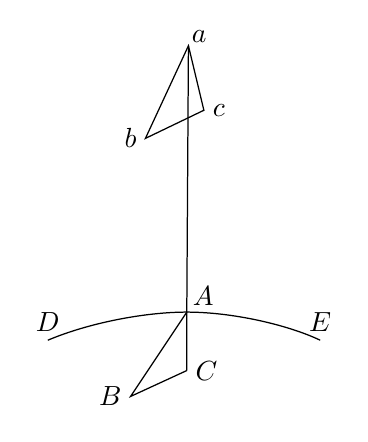
\begin{tikzpicture}[x=.007cm,y=-.007cm,line width=.45pt]
\coordinate (a) at (398,80);
\coordinate (b) at (320,248);
\coordinate (c) at (426,197);
\coordinate (A) at (395,563);
\coordinate (B) at (293,716);
\coordinate (C) at (395,669);
\draw (a)--(A)--(C);
\draw (a)--(b)--(c)--cycle;
\draw (A)--(B)--(C);
\draw (143,614) .. controls (216,583) and (318,563) .. (A)
 .. controls (478,563) and (578,586) .. (637,614);
\node[anchor=south west,inner sep=1pt] at (a) {$a$};
\node[anchor=east,inner sep=3pt] at (b) {$b$};
\node[anchor=west,inner sep=3pt] at (c) {$c$};
\node[anchor=south west,inner sep=2pt] at (A) {$A$};
\node[anchor=east,inner sep=3pt] at (B) {$B$};
\node[anchor=west,inner sep=3pt] at (C) {$C$};
\node[anchor=south,inner sep=3pt] at (143,614) {$D$};
\node[anchor=south,inner sep=3pt] at (637,614) {$E$};
\end{tikzpicture}
\end{center}
This, however, is \textls[150]{insufficient} for judging the difference in the direction of gravity (the plumb line) observed at $A$ and $a$ relative to the equator, since we have no grounds for assuming that $ab$ is parallel to $AB$. The difference between the directions of $ab$ and $AB$ is in fact of the same order as the difference between the angles $BAC$ and $bac$ arising from the two causes you cite. At first glance one would be inclined to suppose that the two straight lines $AB$ and $ab$, extended indefinitely in both directions, would intersect below rather than above, in which case this third cause would act in the same sense, namely by making the altitude of the pole at $a$ greater than at $A$. A more searching investigation, however, shows that this presumption is false and that $ab$ makes a greater, not a smaller, angle with $aAC$ than $AB$ does with $AC$. The third cause therefore acts \textls[150]{against} the first two, and the magnitudes must be worked out to establish whether the altitude of the pole at $a$ might actually be smaller than at $A$.

At the time I lacked the leisure for such an investigation, quite apart from the poor state of my health. However, as soon as I was able to do so, I carried out the investigation for the case in which the Earth is treated as homogeneous. The result was that the altitude of the pole at $a$ is
\[
206\,265''\cdot\frac s{a_0}\sin2\varphi\cdot K
\]
greater than at $A$, where $a_0$ denotes the radius of the equator, $s$ the height $Aa$

\clearpage
\noindent\mbox{}\hfill VARIATION OF THE ALTITUDE OF THE POLE WITH HEIGHT.\hfill 101\par
\noindent in the figure above, $\varphi$ the altitude of the pole at $A$, and $K$ a coefficient that, on the assumption of homogeneity, simply equals the flattening $=\theta$. It is in any case accurate only to the first order of the flattening, which is quite sufficient here. I add that this $K$ may be regarded as made up of three parts: $+\tfrac25\theta$ because $bc>BC$, $+\tfrac45\theta$ because $ab<AB$, and $-\tfrac15\theta$ because $ab$ and $AB$ are not parallel. I did not, however, wish to communicate this result to you immediately, as I wanted to make the investigation independent of the assumption that the Earth is homogeneous. It is of course impossible to obtain a result entirely free of assumptions. I wanted my further investigation to rest solely on the assumption that has as its basis (in one form or another) the famous theorem of \textsc{Clairaut},
\[
\tfrac52\frac hg=\theta+\frac{g'-g}g
\]
where $g$ and $g'$ denote gravity at the equator and the pole, and $h$ the centrifugal force at the equator. The validity of this theorem depends on treating the body of the Earth as composed of similar layers (the density being the same at all points in any one layer, but varying arbitrarily between different layers), or merely assuming that the Earth is an elliptic spheroid, or, thirdly, assuming only that the increase in pendulum length from the equator to the pole is proportional to the square of the sine of the altitude of the pole. In all cases quantities of the second order in the flattening are disregarded.

I have now also carried out this further investigation, though not exactly in the form of a result composed of the three parts mentioned, which can nevertheless be recognized in it. Here the three parts no longer stand in the ratio of the numbers $+2$, $+4$, and $-1$. The third will correspond to a more complicated expression. Remarkably, however, the final result is very simple, namely
\[
K=\frac{g'-g}g,
\]
which thus includes the preceding special case, since, as is well known, for a homogeneous Earth
% Continues on printed 102.
